\documentclass{article}
\usepackage{amsmath}
\usepackage{amssymb}
\usepackage[a4paper, top=25mm, bottom=25mm, left=25mm, right=25mm]{geometry}
\usepackage{pgfplots}
\pgfplotsset{compat=1.18}
\usepackage{mathtools}
\usepgfplotslibrary{polar}
\usepgfplotslibrary{fillbetween}
\usepackage{tikz}
\usetikzlibrary{arrows.meta}

\begin{document}
\pagestyle{empty}
\large

\begin{center}
2019-2020 Spring \\MAT124 Resit\\(01/07/2020)
\end{center}

\noindent 1. The temperature $T$ at the point $(x,y,z)$ in a region of space is given by the formula $T=100-xy-xz-yz$. Find the lowest temperature on the plane $x+y+z=10$.

\hfill

\noindent 2. Show that if $z=f(r, \theta)$, where $r$ and $\theta$ are defined as functions of $x$ and $y$ by the equations $x=r\cos\theta$ and $y=r\sin\theta$, then the equation $\displaystyle\frac{\partial^2z}{\partial x^2}+\frac{\partial ^2z}{\partial y^2} = 0$ becomes

\begin{equation*}
    \frac{\partial^2z}{\partial r^2}+\frac{1}{r^2}\frac{\partial^2z}{\partial\theta^2}+\frac{1}{r}\frac{\partial z}{\partial r}  = 0\:.
\end{equation*}

\hfill

\noindent 3. Evaluate the integral $\displaystyle \int_0^1\int_{\sqrt y}^1 \sqrt{1-x^3}\,dx\,dy$.

\hfill

\noindent 4. Evaluate

\[\displaystyle \int_2^4\int_2^y\,dx\,dy + \int_4^8\int_2^{16/y}\,dx\,dy\]

\hfill

\noindent by reversing the order of integration.

\hfill

\noindent 5. Use a double integral to find the area inside the circle $r=\cos\theta$ and outside the cardioid $r=1-\cos\theta$.

\hfill

\noindent 6. Use polar coordinates to evaluate the double integral

\[\displaystyle\iint_D\sin\left(x^2+y^2\right)\,dA,\]

\hfill

\noindent where $D$ is the region bounded by the circles $x^2+y^2=1$ and $x^2+y^2=4$ and the lines $y=0$, $x=\sqrt3 y$.

\hfill

\noindent 7. Using cylindrical coordinates, evaluate

\[\iiint_D\frac{dV}{x^2+y^2+z^2},\]

\hfill

\noindent where $D$ is the solid region bounded below by the paraboloid $2z=x^2+y^2$ and above by the sphere $x^2+y^2+z^2=8$.

\hfill

\noindent 8. Using spherical coordinates, evaluate the triple integral

\[\iiint_D\sqrt{x^2+y^2+z^2}\,dV,\]

\hfill

\noindent where $D$ is the portion of the solid sphere $x^2+y^2+z^2\leq1$ that lies in the first octant.

\newpage

\begin{center}
2019-2020 Spring Resit (01/07/2020) Solutions\\
(Last update: 8/8/25 (8th of August) 10:44 PM)
\end{center}

\noindent 1) Let $g(x,y,z)=x+y+z-10$ and then, solve the system of equations below using the method of Lagrange multipliers.

\[
\left.
\begin{array}{ll}
\displaystyle\nabla T =\lambda \nabla g\\
\displaystyle g(x,y,z) = 0
\end{array}
\right\}\quad
\nabla T = \left\langle-y-z,-x-z,-x-y\right\rangle=\lambda\left\langle1,1,1\right\rangle= \lambda\nabla g
\]

\begin{align*}T_x+T_y + T_z&=(-y-z) +(-x-z) +(-x-y)=-2x-2y-2z\\&=\lambda+\lambda+\lambda=3\lambda\implies x+y+z=\frac{-3\lambda}{2}\end{align*}

\hfill

\noindent Use the constraint to find the value of $\lambda$.

\[g(x,y,z) = 0 \implies \frac{-3\lambda}{2}-10=0\implies \lambda=-\frac{20}{3}\]

\hfill

\noindent So far, we have the equations below. Solve the system of equations and find the values of $x,y,z$ one by one.

\[
\left.
\begin{array}{ll}
\displaystyle -y-z=-\frac{20}{3}&(1)\\[0.5cm]
\displaystyle -x-z=-\frac{20}{3}&(2)\\[0.5cm]
\displaystyle -x-y=-\frac{20}{3}&(3)
\end{array}
\right\}\quad
\begin{array}{ll}
\displaystyle (1)\:\&\:(2)\rightarrow x-y=0 & (4) \\[0.2cm]
\displaystyle (3)\:\&\:(4)\rightarrow y=\frac{10}{3}&(5)\\[0.5cm]
\displaystyle\therefore z=\frac{10}{3},\quad x=\frac{10}{3}
\end{array}
\]

\hfill

\noindent We now have all the values. Substitute in $T(x,y,z)$ to find the minimum value of the temperature.

\[T_{\text{min}}=T\left(\frac{10}{3},\frac{10}{3},\frac{10}{3}\right)=100-\left(\frac{10}{3}\right)^2-\left(\frac{10}{3}\right)^2-\left(\frac{10}{3}\right)^2=\boxed{\frac{200}{3}}\]

\hfill

\noindent 2) We have $x=r\cos\theta$ and $y=r\sin\theta$.

\[x^2=r^2\cos^2\theta,\quad y^2 =r^2\sin^2\theta\implies x^2+y^2=r^2\left(\cos^2\theta+\sin^2\theta\right)=r^2, \quad \therefore  r=\sqrt{x^2+y^2}\]

\[\frac{y}{x}=\frac{r\sin\theta}{r\cos\theta}=\tan\theta \implies \theta=\tan^{-1}\frac{y}{x}\]

\hfill

\noindent Compute the first-order partial derivatives.

\[\frac{\partial z}{\partial x}=\frac{\partial z}{\partial r}\cdot\frac{\partial r}{\partial x}+\frac{\partial z}{\partial \theta}\cdot\frac{\partial\theta}{\partial x},\quad\quad\frac{\partial z}{\partial y}=\frac{\partial z}{\partial r}\cdot\frac{\partial r}{\partial y} + \frac{\partial z}{\partial\theta}\cdot\frac{\partial\theta}{\partial y}\]

\hfill

\[\frac{\partial r}{\partial x}=\frac{x}{\sqrt{x^2+y^2}}=\cos\theta,\quad\quad\frac{\partial r}{\partial y}=\frac{y}{\sqrt{x^2+y^2}}=\sin\theta\]

\newpage

\[\quad\frac{\partial\theta}{\partial x}=\frac{1}{\displaystyle 1+\frac{y^2}{x^2}}\cdot \left(-\frac{y}{x^2}\right)=\frac{-y}{x^2+y^2}=\frac{-\sin\theta}{r},\quad\quad\frac{\partial\theta}{\partial y}=\frac{1}{\displaystyle1+\frac{y^2}{x^2}}\cdot\frac{1}{x}=\frac{x}{x^2+y^2}=\frac{\cos\theta}{r}\]

\hfill

\noindent Rewrite $\displaystyle\frac{\partial z}{\partial x}$ and $\displaystyle\frac{\partial z}{\partial y}$.

\[\frac{\partial z}{\partial x}=\frac{\partial z}{\partial r}\cdot\frac{x}{\sqrt{x^2+y^2}}+\frac{\partial z}{\partial\theta}\cdot\frac{-y}{x^2+y^2},\quad\quad\frac{\partial z}{\partial y}=\frac{\partial z}{\partial r}\cdot\frac{y}{\sqrt{x^2+y^2}}+\frac{\partial z}{\partial \theta}\cdot\frac{x}{x^2+y^2}\]

\hfill

\noindent Compute the second-order partial derivatives.

\[\frac{\partial}{\partial x}\left(\frac{\partial z}{\partial x}\right)=\frac{\partial}{\partial x}\left(\frac{\partial z}{\partial r}\cdot\frac{x}{\sqrt{x^2+y^2}}+\frac{\partial z}{\partial\theta}\cdot\frac{-y}{x^2+y^2}\right)\]

\begin{align*}\frac{\partial^2z}{\partial x^2}=&\left[\left(\frac{\partial^2z}{\partial r^2}\cdot\frac{\partial r}{\partial x}+\frac{\partial^2 z}{\partial\theta\,\partial r}\cdot\frac{\partial\theta}{\partial x}\right)\cdot\frac{x}{\sqrt{x^2+y^2}}+\frac{\partial z}{\partial r}\cdot\frac{1\cdot\sqrt{x^2+y^2}-x\cdot\frac{x}{\sqrt{x^2+y^2}}}{\left(\sqrt{x^2+y^2}\right)^2}\right]\\&+\left[\left(\frac{\partial^2z}{\partial \theta^2}\cdot\frac{\partial \theta}{\partial x}+\frac{\partial^2 z}{\partial r\,\partial \theta}\cdot\frac{\partial r}{\partial x}\right)\cdot\frac{-y}{x^2+y^2}+\frac{\partial z}{\partial\theta}\cdot\frac{y}{(x^2+y^2)^2}\cdot2x\right]\end{align*}

\hfill

\[\frac{\partial}{\partial y}\left(\frac{\partial z}{\partial y}\right)=\frac{\partial}{\partial y}\left(\frac{\partial z}{\partial r}\cdot\frac{y}{\sqrt{x^2+y^2}}+\frac{\partial z}{\partial \theta}\cdot\frac{x}{x^2+y^2}\right)\]

\begin{align*}\frac{\partial^2z}{\partial y^2}=&\left[\left(\frac{\partial^2z}{\partial r^2}\cdot\frac{\partial r}{\partial y}+\frac{\partial^2 z}{\partial\theta\,\partial r}\cdot\frac{\partial\theta}{\partial y}\right)\cdot\frac{y}{\sqrt{x^2+y^2}}+\frac{\partial z}{\partial r}\cdot\frac{1\cdot\sqrt{x^2+y^2}-y\cdot\frac{y}{\sqrt{x^2+y^2}}}{\left(\sqrt{x^2+y^2}\right)^2}\right]\\&+\left[\left(\frac{\partial^2z}{\partial \theta^2}\cdot\frac{\partial \theta}{\partial y}+\frac{\partial^2 z}{\partial r\,\partial \theta}\cdot\frac{\partial r}{\partial y}\right)\cdot\frac{x}{x^2+y^2}+\frac{\partial z}{\partial\theta}\cdot\frac{-x}{(x^2+y^2)^2}\cdot2y\right]\end{align*}

\hfill

\noindent Add the second-order partial derivatives and set to $0$. The last terms eliminate each other. Write $x$ and $y$ in terms of $r$ and $\theta$.

\begin{align*}\frac{\partial^2 z}{\partial x^2}+\frac{\partial^2 z}{\partial y^2}=&\left[\left(\frac{\partial^2z}{\partial r^2}\cdot\cos\theta +\frac{\partial^2z}{\partial\theta\,\partial r}\cdot\frac{-\sin\theta}{r}\right)\cdot\cos\theta+\frac{\partial z}{\partial r}\cdot\frac{\sin^2\theta}{r}\right]\\\\&+\left[\left(\frac{\partial^2z}{\partial\theta^2}\cdot\frac{-\sin\theta}{r} + \frac{\partial^2z}{\partial r\,\partial\theta}\cdot\cos\theta\right)\cdot\frac{-\sin\theta}{r}\right]\\\\&+\left[\left(\frac{\partial^2z}{\partial r^2}\cdot\sin\theta +\frac{\partial^2z}{\partial\theta\,\partial r}\cdot\frac{\cos\theta}{r}\right)\cdot\sin\theta+\frac{\partial z}{\partial r}\cdot\frac{\cos^2\theta}{r}\right]\\\\&+\left[\left(\frac{\partial^2z}{\partial\theta^2}\cdot\frac{\cos\theta}{r} + \frac{\partial^2z}{\partial r\,\partial\theta}\cdot\sin\theta\right)\cdot\frac{\cos\theta}{r}\right]=0\end{align*}

\newpage

\noindent Inspect the terms that add up to $0$. Recall $\sin^2\theta+\cos^2\theta=1$, then the equation reduces to

\begin{align*}
\frac{\partial^2z}{\partial x^2}+\frac{\partial^2z}{\partial y^2}&=\frac{\partial^2z}{\partial r^2}\cdot\left(\cos^2\theta+\sin^2\theta\right)+\frac{\partial z}{\partial r}\cdot\frac{\sin^2\theta+\cos^2\theta}{r}+\frac{\partial^2z}{\partial\theta^2}\cdot\left(\sin^2\theta+\cos^2\theta\right)\\\\&=\frac{\partial^2z}{\partial r^2}+\frac1r\cdot\frac{\partial z}{\partial r}+\frac{\partial^2z}{\partial\theta^2}=0,
\end{align*}

\hfill

\noindent which we set out to demonstrate.

\hfill

\noindent 3) Change the order of integration using the graph below and then evaluate the integral.

\begin{center}
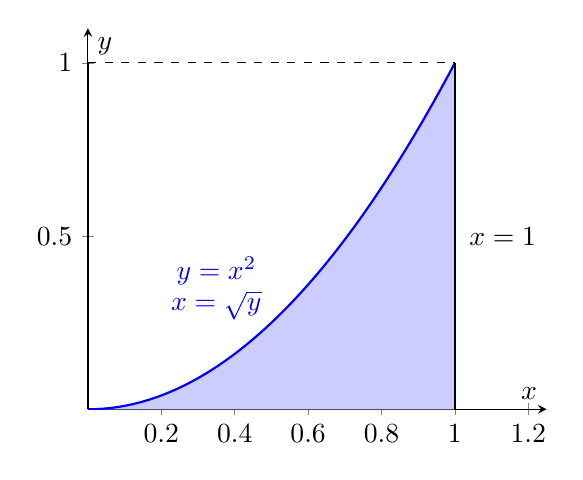
\begin{tikzpicture}
  \begin{axis}[
      axis lines = middle,
      xlabel = $x$, ylabel = $y$,
      domain=0:1,
      ymin=0, ymax=1.1,
      xmin=0, xmax=1.25,
      samples=100,
      clip=true,
      scale=0.85
    ]
    
    \addplot [
      name path=A,
      domain=0:1,
      draw=none,
    ] {x^2};

    \path[name path=B] (axis cs:0,1) -- (axis cs:1,1);
    \path[name path=C] (axis cs:0,0) -- (axis cs:0,1);
    \path[name path=D] (axis cs:0,0) -- (axis cs:1,0);

    \addplot [
      fill=blue!20,
      draw=none,
    ] fill between [
      of=A and D,
      soft clip={domain=0:1},
    ];
    
    \addplot[blue, thick] {x^2};
    \addplot[black, thick] coordinates {(0,0) (0,1)};
    \addplot[black, thick] coordinates {(1,0) (1,1)};
    \draw[dashed] (axis cs: 0,1) -- (axis cs: 1,1);
    \node at (axis cs: 1.13, 0.5) {$x=1$};
    \node[blue] at (axis cs: 0.35, 0.4) {$y=x^2$};
    \node[blue] at (axis cs: 0.35, 0.3) {$x=\sqrt{y}$};

  \end{axis}
\end{tikzpicture}
\end{center}
\begin{align*}
\int_0^1\int_{\sqrt{y}}^1\sqrt{1-x^3}\,dx\,dy&=\int_0^1\int_0^{x^2}\sqrt{1-x^3}\,dy\,dx=\int_0^1x^2\sqrt{1-x^3}\,dx\:\left[\begin{array}{c}u=1-x^3 \\du=-3x^2\,dx\end{array}\right]\\\\&=\int\frac{\sqrt{u}}{-3}\,du=-\frac29u^{3/2}+c=-\frac29\left(1-x^3\right)^{3/2}\Bigg|_0^1=0-\left[-\frac29\right]=\boxed{\frac29}\end{align*}

\hfill

\noindent 4)

\begin{minipage}{0.45\textwidth}
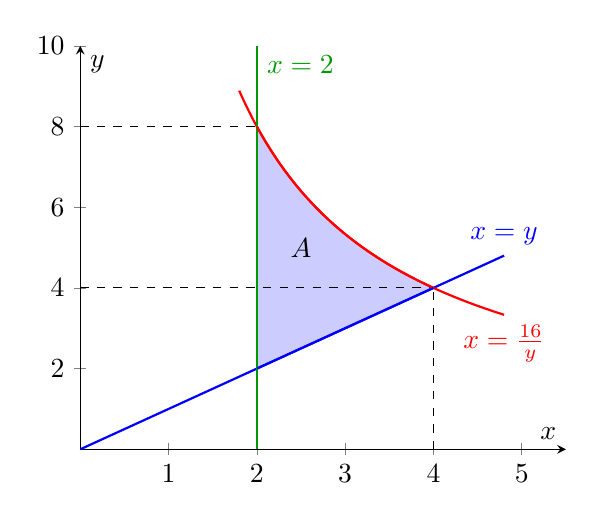
\begin{tikzpicture}
  \begin{axis}[
      axis lines = center,
      xlabel = {$x$},
      ylabel = {$y$},
      domain=1:4,
      samples=200,
      ymin=0, ymax=10,
      xmin=0, xmax=5.5,
      clip=true,
      scale=0.9
    ]
    
    \draw[dashed] (axis cs: 0,4) -- (axis cs: 4,4);
    \draw[dashed] (axis cs: 4,0) -- (axis cs: 4,4);
    \draw[dashed] (axis cs: 0,8) -- (axis cs:2,8);
    \node at (2.5,5) {$A$};

    \addplot[blue, thick, domain=0:4.8] {x} node[above] {$x = y$};

    \addplot[red, thick, domain=1.8:4.8] {16/x} node[below] {$x = \frac{16}{y}$};

    \addplot[green!60!black, thick, domain=0:10] ({2},x) node[below right] {$x = 2$};
    
    \addplot[red, thick, domain=2:4, name path=A] {16/x};
    \addplot[blue, thick, domain=2:4, name path=B] {x};

    \addplot [
      fill=blue!20,
      draw=none,
    ] fill between [
      of=A and B,
      soft clip={domain=2:4},
    ];
  \end{axis}
\end{tikzpicture}
\end{minipage}\hspace{0.25em}
\begin{minipage}{0.5\textwidth}
\begin{align*}A&=\int_2^4\int_2^y\,dx\,dy + \int_4^8\int_2^{16/y}\,dx\,dy\\\\&=\int_2^4\int_{x}^{\frac{16}x}\,dy\,dx=\int_2^4\left(\frac{16}x-x\right)\,dx\\\\&=\left[16\ln|x| -\frac{x^2}2\right]_2^4\\\\&=\left[\left(16\ln4 -\frac{4^2}{2}\right)-\left(16\ln2-\frac{2^2}{2}\right)\right]\\\\&=\boxed{16\ln2-6}\end{align*}
\end{minipage}

\newpage

\noindent 5)
\begin{center}
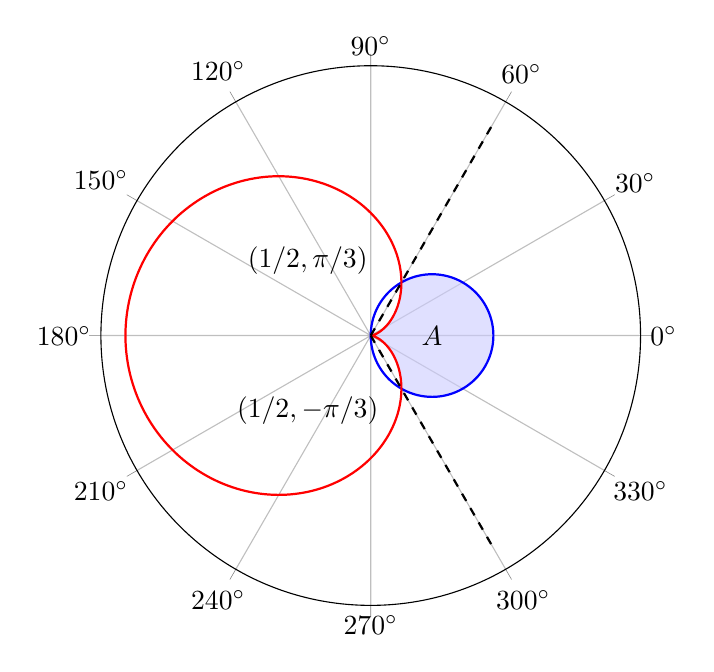
\begin{tikzpicture}
  \begin{polaraxis}[ytick=\empty, axis y line=none, xticklabel=$\pgfmathprintnumber{\tick}^\circ$,]
    \addplot [
      domain=-pi/3:pi/3,
      samples=300,
      draw=none,
      name path=A,
      data cs=polarrad,
    ] {cos(deg(x))};

    \addplot [
      domain=-pi/3:pi/3,
      samples=300,
      draw=none,
      name path=B,
      data cs=polarrad,
    ] {1-cos(deg(x))};

    \addplot [
      blue!20,
      fill opacity=0.6,
    ] fill between[of=A and B];

    \addplot [
      domain=0:2*pi,
      samples=300,
      thick,
      blue,
      data cs=polarrad,
    ] {cos(deg(x))};

    \addplot [
      domain=0:2*pi,
      samples=300,
      thick,
      red,
      data cs=polarrad,
    ] {1-cos(deg(x))};

    \draw[black, thick, dashed] (axis cs: 60,0) -- (axis cs: 60,2);
    \draw[black, thick, dashed] (axis cs: -60,0) -- (axis cs: -60,2);

    \node at (axis cs:130,0.8) {$(1/2,\pi/3)$};
    \node at (axis cs:-130,0.8) {$(1/2,-\pi/3)$};
    \node at (0,0.5) {$A$};

  \end{polaraxis}
\end{tikzpicture}
\end{center}

\begin{align*}
A&=\int_{-\pi/3}^{\pi/3}\int_{1-\cos\theta}^{\cos\theta}\,r\,dr\,d\theta=\frac12\int_{-\pi/3}^{\pi/3}\left[\cos^2\theta-(1-\cos\theta)^2\right]\,d\theta=\frac12\int_{-\pi/3}^{\pi/3}\left(2\cos\theta-1\right)\,d\theta\\\\&=\frac12\bigg[2\sin\theta-\theta\bigg]_{-\pi/3}^{\pi/3}=\frac12\left[\left(2\sin\frac\pi3-\frac\pi3\right)-\left(2\sin\left(-\frac\pi3\right)+\frac\pi3\right)\right]=\boxed{\sqrt3-\frac\pi3}
\end{align*}

\hfill

\noindent 6)
\begin{center}
    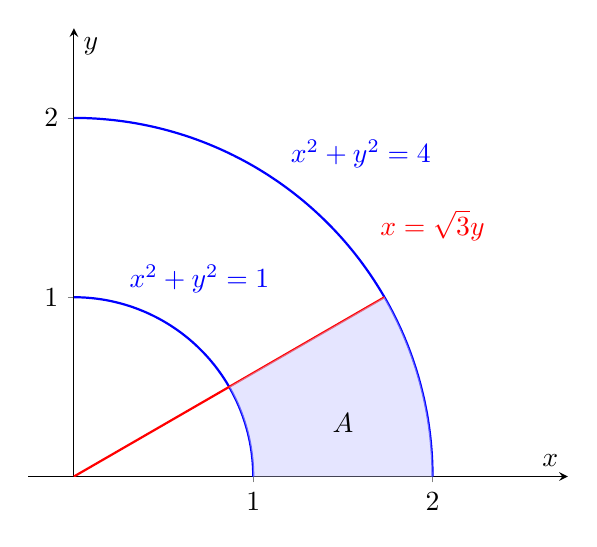
\begin{tikzpicture}
    \begin{axis}[
        axis equal,
        axis lines = center,
        xlabel = $x$,
        ylabel = $y$,
        xmin = 0, xmax = 2.5,
        ymin = 0, ymax = 2.5,
        xtick = {-2,-1,1,2},
        ytick = {-2,-1,1,2},
    ]

    \addplot[domain=0:90, samples=100, blue, thick] ({cos(x)}, {sin(x)});
    \addplot[domain=0:90, samples=100, blue, thick] ({2*cos(x)}, {2*sin(x)});
    \addplot[domain=0:1, red, thick] ({sqrt(3)*x}, {x});
    \fill[blue!20, opacity=0.5] 
        plot[domain=0:30, samples=30,variable=\t] ({2*cos(\t)}, {2*sin(\t)}) -- 
        plot[domain=30:0, samples=30,variable=\t] ({cos(\t)}, {sin(\t)}) -- cycle;
    \node[blue] at (1.6,1.8) {$x^2 + y^2 = 4$};
    \node[blue] at (0.7,1.1) {$x^2 + y^2 = 1$};
    \node[red] at (2,1.4) {$x = \sqrt{3}y$};
    \node at (1.5,0.3) {$A$};

    \end{axis}
\end{tikzpicture}
\end{center}

\noindent Use the following transformation to switch to polar coordinates.

\[
\begin{array}{c}x=r\cos\theta\\y=r\sin\theta\\[0.2cm]x^2+y^2=r^2\\[0.2cm]\displaystyle\theta=\tan^{-1}\frac yx\\[0.2cm]dA=r\,dr\,d\theta
\end{array}\quad\rightarrow\quad
\begin{array}{c}
x^2+y^2=1\,\implies\,r^2=1\implies r=1\\x^2+y^2=4\,\implies\,r^2=4\implies r=2\\y=0\implies\theta=0\\
\displaystyle x=\sqrt3y\implies\tan^{-1}\frac yx=\tan^{-1}\frac1{\sqrt3}\implies\theta=\frac{\pi}6\\\\\displaystyle\therefore 1\leq r\leq2,\quad 0\leq\theta\leq\frac{\pi}6
\end{array}
\]

\newpage

\begin{align*}
\int_0^{\pi/6}\int_1^2\sin(r^2)\,r\,dr\,d\theta&=\int_0^{\pi/6}\left[-\frac12\cos{r^2}\right]_1^2\,d\theta=-\frac12\int_0^{\pi/6}\left(\cos4-\cos1\right)\,d\theta\\\\&=\frac12(\cos1-\cos4)\cdot\theta\,\bigg|_0^{\pi/6}=\boxed{\frac\pi{12}(\cos1-\cos4)}
\end{align*}

\hfill

\noindent 7) For cylindrical coordinates, we have

\[
\begin{array}{c}
z=z\\
r^2=x^2+y^2\\
dV=r\,dz\,dr\,d\theta
\end{array}\quad\rightarrow\quad
\begin{array}{c}
\displaystyle2z=x^2+y^2\,\rightarrow\,z=\frac{r^2}2\\[0.3cm]
x^2+y^2+z^2=8\,\rightarrow\,z=\sqrt{8-r^2}\\
\end{array}
\]

\hfill

\noindent Find where the surfaces $2z=x^2+y^2$ and $x^2+y^2+z^2=8$ intersect to determine the limits of $r$.

\begin{align*}x^2+y^2+z^2=8&\implies 2z + z^2 = 8\implies (z+4)(z-2) = 0\implies z=2\\&\implies4=x^2+y^2=r^2 \implies r=2\end{align*}

\hfill

\noindent The lower limit of $r$ is apparently $0$. The region in the $xy$-plane is circular if we project the domain. Therefore, $0\leq\theta\leq2\pi$. Now, set up the triple integral in polar coordinates.

\begin{align*}\mathrm{I}&=\iiint_D\frac{dV}{x^2+y^2+z^2}=\int_0^{2\pi}\int_0^2\int_{r^2/2}^{\sqrt{8-r^2}}\frac{r}{r^2+z^2}\,dz\,dr\,d\theta\\\\&=\int_0^{2\pi}\int_0^2\int_{r^2/2}^{\sqrt{8-r^2}}\frac{1}{1+\left(\frac zr\right)^2}\cdot\frac1r\,dz\,dr\,d\theta=\int_0^{2\pi}\int_0^2\left[\arctan\left(\frac zr\right)\right]_{r^2/2}^{z=\sqrt{8-r^2}}\,dr\,d\theta\\\\&=\int_0^{2\pi}\int_0^2\arctan\left(\frac{\sqrt{8-r^2}}r\right)\,dr\,d\theta-\int_0^{2\pi}\int_0^2\arctan\left(\frac r2\right)\,dr\,d\theta\end{align*}

\hfill

\noindent $\theta$ is independent of $r$. Therefore, we can write the following.

\begin{equation}
\mathrm{I}=2\pi\int_0^2\arctan\left(\frac{\sqrt{8-r^2}}r\right)\,dr-2\pi\int_0^2\arctan\left(\frac r2\right)\,dr
\end{equation}

\hfill

\noindent Now, use integration by parts for the left-hand integral in $(1)$. Apply the chain rule and the quotient rule rigorously.

\begin{align*}
\displaystyle u=\arctan\left(\frac{\sqrt{8-r^2}}r\right)&\rightarrow\displaystyle du=\frac1{\displaystyle1+\left(\frac{\sqrt{8-r^2}}r\right)^2}\cdot\frac{\displaystyle \frac{1}{2\sqrt{8-r^2}}\cdot(-2r)\cdot r -\sqrt{8-r^2}\cdot 1}{r^2}\,dr\\
\displaystyle dv=dr&\rightarrow v=r
\end{align*}

\newpage

\noindent Notice that we have an improper integral, where we need to use limits.

\begin{align}
\int_0^2\arctan\left(\frac{\sqrt{8-r^2}}r\right)\,dr&=\lim_{T\to0^+}\left[r\cdot\arctan\left(\frac{\sqrt{8-r^2}}r\right)\Bigg|_T^2-\int_T^2r\cdot\frac{-1}{\sqrt{8-r^2}}\,dr\right]\nonumber\\\nonumber\\&=\lim_{T\to0^+}\left[r\cdot\arctan\left(\frac{\sqrt{8-r^2}}r\right)-\sqrt{8-r^2}\right]_T^2
\end{align}

\hfill

\noindent Compute the other integral in $(1)$ using integration by parts.

\begin{align*}
\displaystyle u=\arctan\left(\frac{r}2\right)&\rightarrow\displaystyle du=\frac1{\displaystyle1+\left(\frac{r}2\right)^2}\cdot\frac12\,dr\\
\displaystyle dv=dr&\rightarrow v=r
\end{align*}
\begin{align}
\int_0^2\arctan\left(\frac r2\right)\,dr&=r\cdot\arctan\left(\frac r2\right)\Bigg|_0^2-\int_0^2r\cdot\frac2{4+r^2}\,dr\nonumber\\\nonumber\\&=\left[r\cdot\arctan\left(\frac r 2\right)-\ln\left|4+r^2\right|\right]_0^2
\end{align}

\hfill

\noindent Rewrite $(1)$ using $(2)$ and $(3)$.

\begin{equation*}
\mathrm{I}=2\pi\lim_{T\to0^+}\left[r\cdot\arctan\left(\frac{\sqrt{8-r^2}}r\right)-\sqrt{8-r^2}\right]_T^2-2\pi\left[r\cdot\arctan\left(\frac r2\right)-\ln\left|4+r^2\right|\right]_0^2
\end{equation*}
\begin{align*}
\mathrm{I}=\:&2\pi\left(2\cdot\arctan1-2\right)-2\pi\lim_{T\to0^+}\left[T\cdot\arctan\frac{\sqrt{8-T^2}}T-\sqrt{8-T^2}\right]\\\\&-2\pi\left[\left(2\cdot\arctan1-\ln8\right)-(0-\ln4)\right]
\end{align*}
\begin{equation}
\mathrm{I}=\pi\left(\ln4-4+2\lim_{T\to0^+}\left(\sqrt{8-T^2}\right)\right)-2\pi\lim_{T\to0^+}\left(T\cdot\arctan\frac{\sqrt{8-T^2}}T\right)
\end{equation}

\hfill

\noindent We need to evaluate the limit on the right side in $(4)$ using the squeeze theorem.

\[-\frac\pi2\leq\arctan\left(\frac{\sqrt{8-T^2}}T\right)\leq\frac\pi2\]
\[-\frac{T\cdot\pi}2\leq T\cdot\arctan\left(\frac{\sqrt{8-T^2}}T\right)\leq\frac{T\cdot\pi}2\]
\[\lim_{T\to0^+}\frac{-T\cdot\pi}2=\lim_{T\to0^+}\frac{T\cdot\pi}2=0\implies\lim_{T\to0^+}\left(T\cdot\arctan\frac{\sqrt{8-T^2}}T\right)=0\]

\newpage

\noindent The limit on the left side in $(4)$ is simply equal to $2\sqrt2$. The value of the integral is then

\[\boxed{\mathrm{I}=\pi\left(\ln4-4+4\sqrt2\right)}\]

\hfill

\noindent 8) For spherical coordinates, we have

\[
\begin{array}{c}
z=\rho\cos\phi\\
r=\rho\sin\phi\\
x^2+y^2+z^2=\rho^2\\
dV=\rho^2\sin\phi\,d\rho\,d\phi\,d\theta
\end{array}\quad\rightarrow\quad
\begin{array}{c}
x^2+y^2+z^2\leq1\,\implies\,\rho^2\leq1\,\implies\,0\leq\rho\leq1\\
\sqrt{x^2+y^2+z^2}=1\,\rightarrow\,\sqrt{\rho^2}=1\implies\rho=1\\\\
\displaystyle\therefore0\leq\theta\leq\frac\pi2,\quad0\leq\phi\leq\frac\pi2
\end{array}
\]

\hfill

\noindent Set up the integral and then evaluate.

\begin{align*}
\mathrm{I}&=\iiint_D\sqrt{x^2+y^2+z^2}\,dV=\int_0^{\pi/2}\int_0^{\pi/2}\int_0^1\rho\cdot\rho^2\sin\phi\,d\rho\,d\phi\,d\theta\\\\&=\int_0^{\pi/2}\int_0^{\pi/2}\left[\frac{\rho^4}4\right]_{\rho=0}^{\rho=1}\sin\phi\,d\phi\,d\theta=\frac14\int_0^{\pi/2}\int_0^{\pi/2}\sin\phi\,d\phi\,d\theta=\frac14\int_0^{\pi/2}\bigg[-\cos\phi\bigg]_0^{\pi/2}\,d\theta\\\\&=\frac14\int_0^{\pi/2}\,d\theta=\boxed{\frac\pi8}
\end{align*}

\end{document}